\section{Network Simulation and Topologies}
Because this work places a particular emphasis on network optimization, the network simulation component of FaaS-Sim is of particular relevancy to us.
Under the hood, FaaS-Sim relies on Ether\cite{rausch-ether} for its networking.

Aside from vast option for customization, Ether supports a number of networking primitives that allow us to easily create a range of topologies.
In Ether's model, resources are usually, but not necessarily, grouped together in a cell.
The most important ones for our case are the \textit{LAN Cell} and the \textit{Shared Link Cell}.
The LAN Cell represents a set of compute nodes which are interconnected with each other in the way a LAN typically is, which means bandwidth is high, latency low, and variance small.\\
Contrary to that Shared Link Cells are more typical of what we might expect in an IoT scenario. 
It represents multiple nodes, which, as the name suggests, share a network connection between them.
This can, for example, be used to represent a number of edge devices which are grouped together into a small compute box and share a mobile internet connection for wider connectivity.

The networking simulation in Ether is based around the \textit{Link} object\cite{rausch-ether}, which represents a connection between nodes.
A mobile network connection, for example, would be considered a Link.
As Links represent connections, they also have a set bandwidth and latency.
To more accurately simulate how networks behave in real life, the latency of a link is not defined as a fixed number, but as a random distribution which gets sampled during simulation.

% decided to do a textual representation, as it was more useful
% this is just a placeholder in case I change my mind

To simulate network transfers Ether uses a flow-based simulation.
The transfer of a request from one node to another is considered a flow.
For each flow two steps are simulated: TCP connection establishment, and data transfer.
TCP connection establishment is assumed to be equal to $ 3 \cdot \text{latency}$ of the route the flow takes, based on the three-way SYN, SYN-ACK, ACK handshake of the TCP protocol.\\
The data transfer is where the flow simulation component is used.
Each flow consists of a number of hops, connected by links.
Each of these links has a set latency, bandwidth, and potentially a number of other flows currently being transferred.
To calculate how long data transfer takes, we first determine the bandwidth.
The bandwidth is determined by the minimum bandwidth available from any of the flow's links.
What exactly this is depends on the general bandwidth of the link in question, and by how many flows have to share this available bandwidth.
Once the bandwidth of the flow is determined we can simply calculate how long data transfer will take, given a request of known size.
To preserve the impact different flows have on each other, once a flow is added to the system, or once a flow is completed and thus removed, every link of the flow is updated and potentially recalculates the bandwidth of other running flows.
Other flows might be unaffected, but may also see and increase or decrease in available bandwidth depending on whether there are now more or fewer flows competing.
If flows are competing for bandwidth, they are all treated with equal priority, and share equally in the available bandwidth.


The topologies we use for our evaluations are based on the concept of smart cities\cite{suSmartCityApplications2011}.
In this context we assume there may or may not be a central point in the city which provides a high amount of computational capability, i.e. a data center, and that the majority of computational capability will be interspersed throughout the city alongside with the clients.

For these edge-located resources we assume that two major types exist: \textit{Smart Poles} and \textit{\gls{ran} Towers}.
We consider \gls{ran} Towers to be any type of LTE or 5G mobile base station, which in our smart city scenario would additionally be equipped with edge computing capability.
The Smart Poles we consider to be a functionally similar, though comparatively smaller device, much like the Huawei PoleStar\cite{huaweiPolestar}, which is also equipped with computational capability, albeit less of it, and providing a connection to the wider network.
We assume that these Smart Poles would be spread out throughout the city like sensor nodes in the Array of Things\cite{catlettArrayThingsScientific2017a}, a real world edge computing and smart city sensing deployment.
In terms of latency and bandwidth we assume latency to Smart Pole devices to be in the same ballpark as WiFi connections, while \gls{ran} Tower connections are in line with what one would typically expect of LTE or 5G connections respectively.
In keeping with our methodology of informing simulation values with real world measurements where possible, we used the research conducted by Braud et al.\cite{braudMulticarrierMeasurementStudy2019} and Nikravesh et al.\cite{nikraveshMobileNetworkPerformance2014a} on real world LTE network characteristics to inform our parametrization of these connections.
We also assume that truly low latency connections for client devices are only provided by physically near access points such as the aforementioned Smart Pole devices, as research on wireless network technology indicates that there is a fundamental tradeoff between bandwidth, latency, and reliability\cite{soretFundamentalTradeoffsReliability2014}.

\begin{figure}
    \centering
    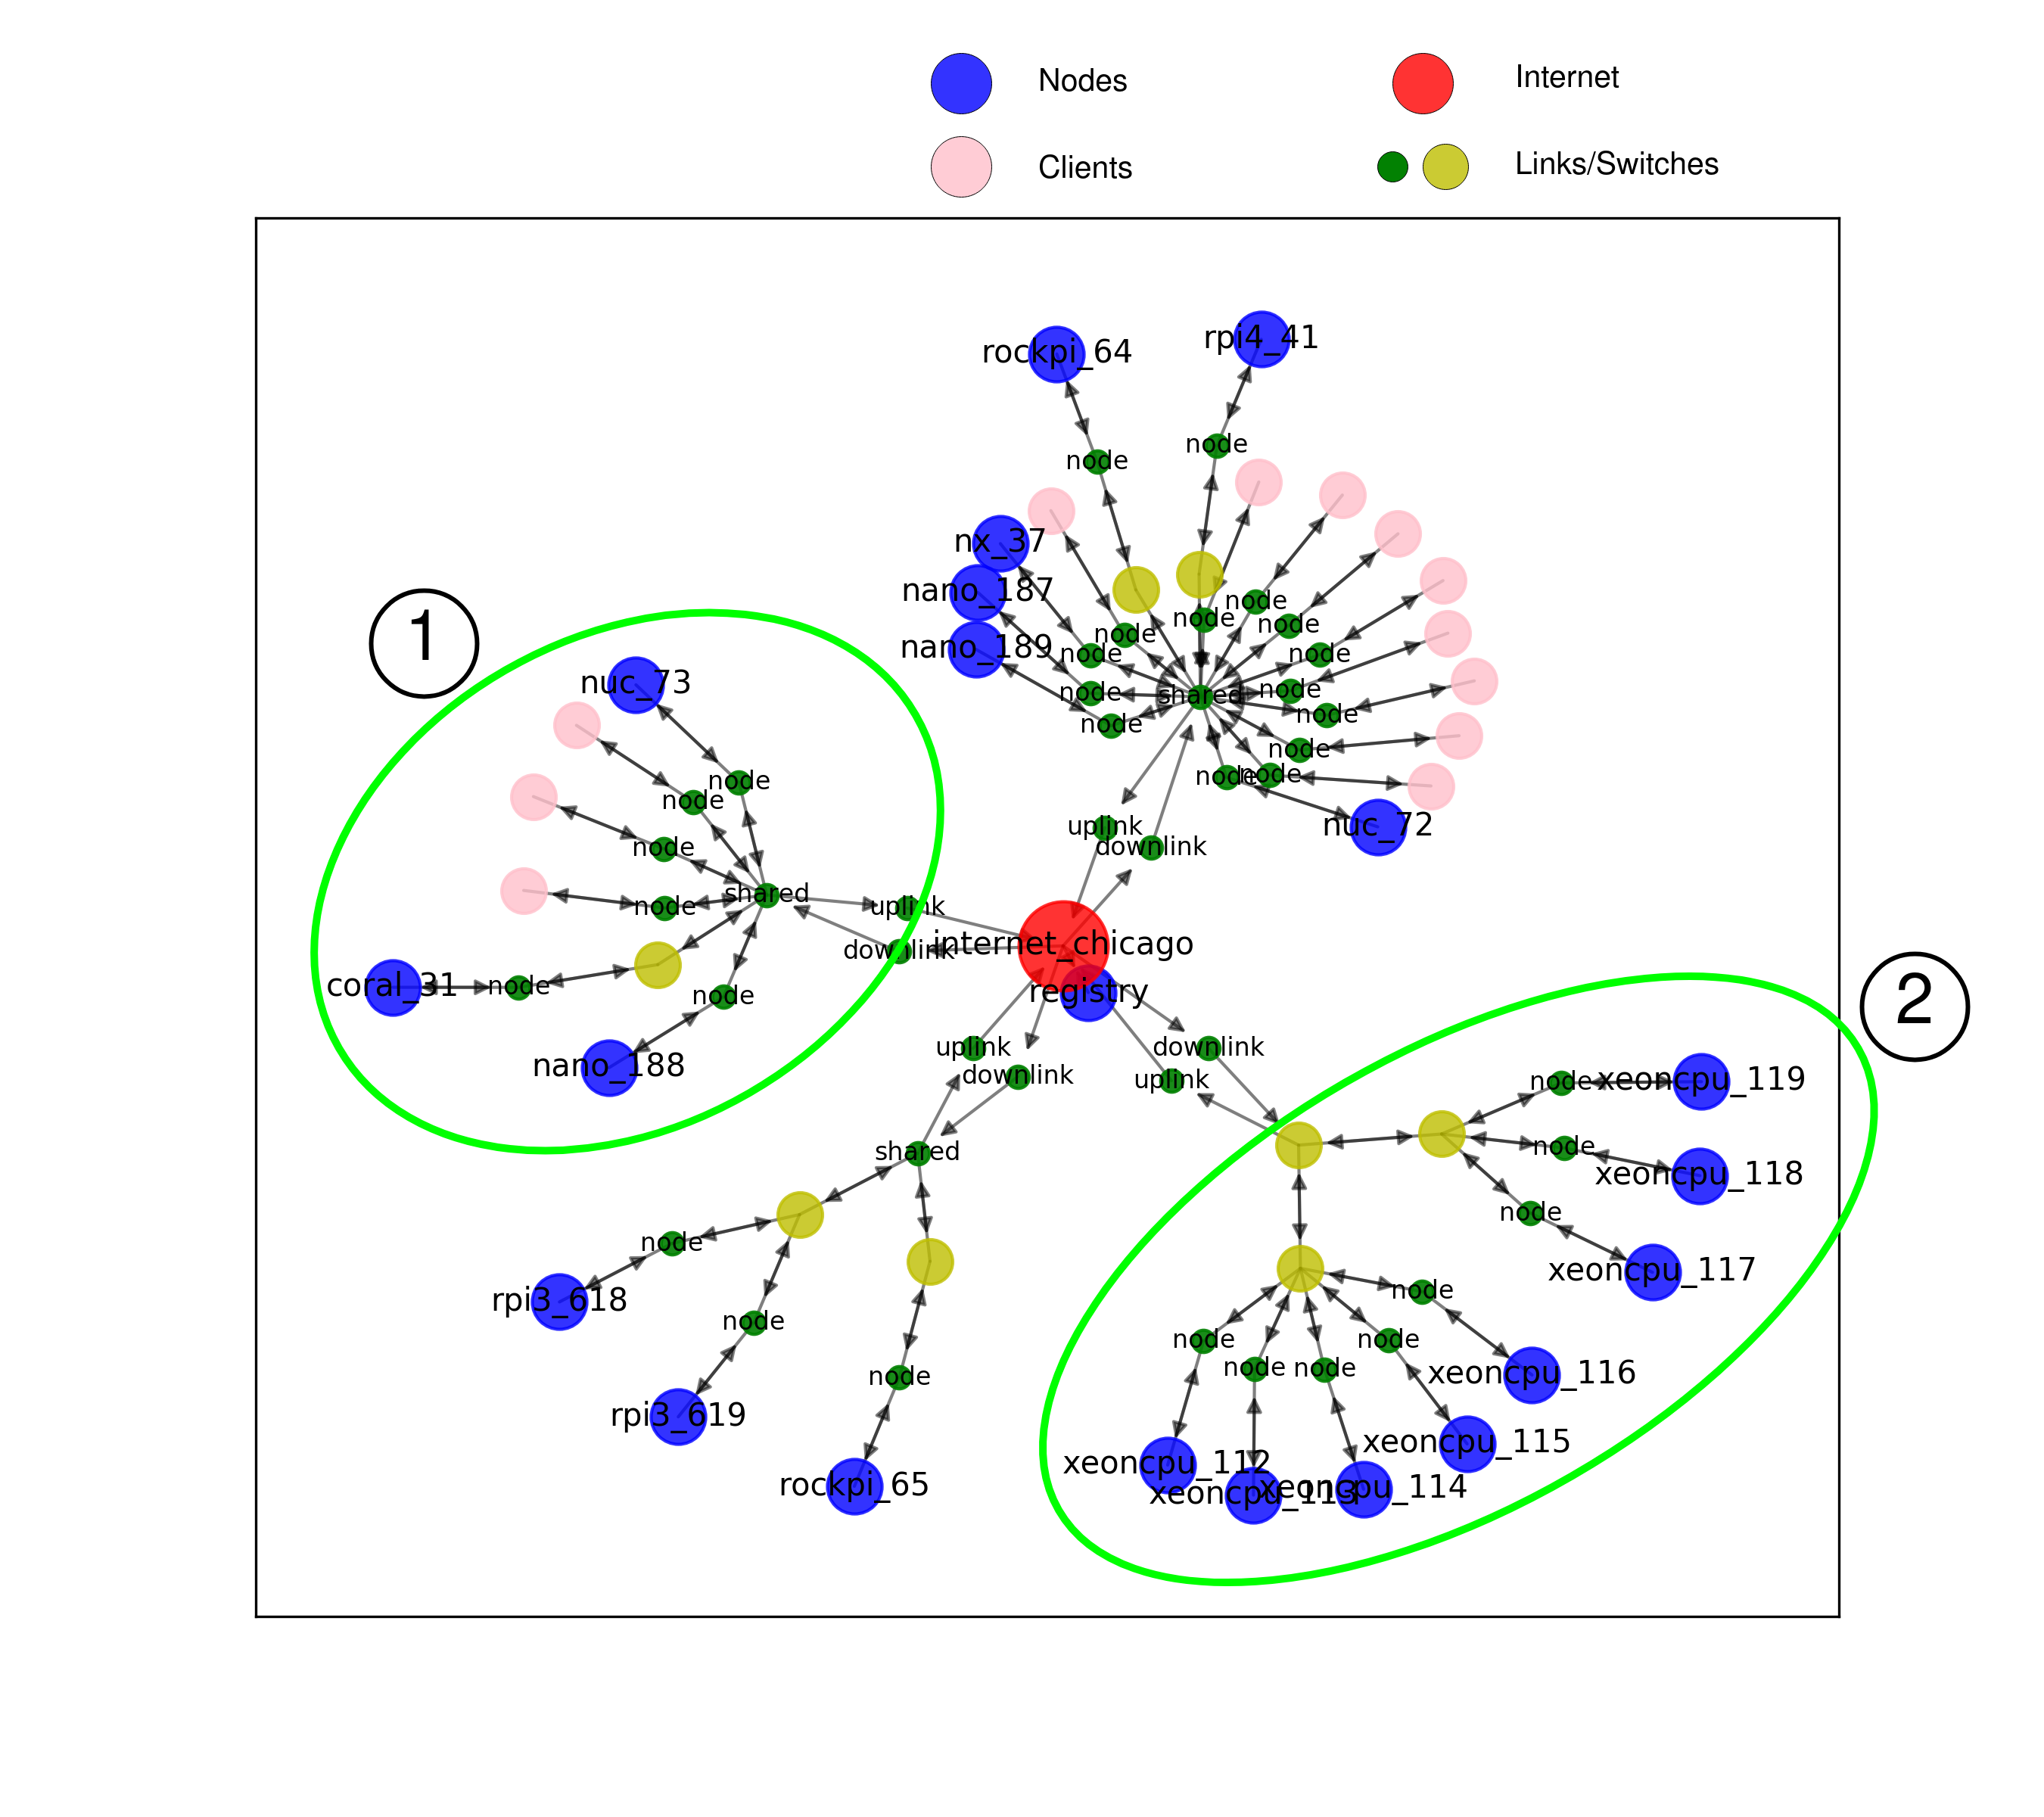
\includegraphics[width=\linewidth]{graphics/diagrams/tiny_topo.png}
    \caption{Simplified network topology of a single smart city. Centered around the internet backbone uplink (red), 1) shows edge devices co-located with client devices. 2) shows a small cloud data center or cloudlet. Note the lack of clients directly connected to the cloudlet.}
    \label{fig:tiny_topo}
\end{figure}

Finally, Figure \ref{fig:tiny_topo} shows a simplified visualization of how one of our smart city topologies is structured.
Note that latency cannot be read from this visualization and that distances between nodes on the visualization do not correspond to network distances whatsoever.
The wider internet, presented as a red circle, is how communication to areas not deemed within the city, or general web-services such as container registries would be routed.
Also note that we only represent logical network links and connections in our topologies, which means that while in truth there might be tens of network hops between an edge node and the wider internet (e.g. through the nearest backbone uplink), for simulation performance reasons we do not include these in our model.